\section{Mise en contexte bibliographique}\label{sec:mise-en-contexte-bibliographique}
   \subsection{GNSS : les origines}\label{subsec:gnss-les-origines}
      Les GNSS (\textit{Global Navigation Satellite Systems}) sont des constellations de satellites conçues afin de fournir un positionnement et un chronométrage d'informations à destination des utilisateurs aussi bien sur Terre que dans l'espace.
      Ils sont utilisés pour générer une estimation de la position, de la vitesse et du temps en traitant les signaux transmis par des satellites d'orbites connues.

      Il existe de nos jours quatre types de systèmes GNSS : GPS, GLONASS, GALILEO et BEIDOU~\cite{gebre-egziabherGNSSApplicationsMethods2009}.

      \subsubsection{Le GPS}
         Actuellement, la constellation la plus utilisée à l'échelle mondiale est le GPS (\textit{Global Positioning System}), conçu par le département de la défense des États-Unis à des fins militaires.
         Le déploiement du système GPS a débuté le 22 février 1978 avec le lancement du premier satellite \textit{Bloc I Navstar GPS}.
         Sa capacité opérationnelle initiale a été annoncée en décembre 1993, pas moins de 24 satellites GPS répartis sur 6 orbites.

      \subsubsection{Le GLONASS}
         En supplément du GPS, un autre système pleinement opérationnel est le GLONASS (\textit{\foreignlanguage{russian}{глобальная навигационная спутниковая система}, Globalnaïa Navigatsionnaïa Spoutnikovaïa Sistéma}) de la Fédération de Russie.
         Ce programme, né dans les années 1980, est devenu opérationnel en 1995 avec une constellation également composée de 24 satellites sur 6 orbites.

         Cependant, la chute de l'URSS a entraîné une baisse drastique des fonds alloués au système GLONASS ayant pour conséquence sa dégradation.
         Depuis 2001, on compte au nombre de 6 les satellites encore opérationnels.

      \subsubsection{Galileo}
         L'Europe, cherchant à affirmer sa souveraineté, tente de s'affranchir des systèmes GPS et GLONASS au travers du projet Galileo, imaginé entre 1999 et 2000 par 4 membres de l'Union Européenne (France, Allemagne, Italie et Royaume-Uni).

         Le système Galileo devrait être opérationnel à l'horizon 2024, fort d'une constellation de 30 satellites répartis sur 3 orbites.

      \subsubsection{Beidou}
         La Chine a également mis en place, à partir de 2000, son propre GNSS appelé Beidou (\textit{\begin{CJK}{UTF8}{gbsn}北斗\end{CJK}}).
         Cette constellation est pleinement opérationnelle depuis le 23 juin 2020, totalisant 35 satellites sur 3 orbites.

   \subsection{Applications}\label{subsec:applications}
      Des applications pratiques des GNSS se retrouvent dans un large spectre de domaines, aussi bien pour des problématiques de positionnement que de synchronicité temporelle.

      On présente alors une liste non exhaustive de domaines et d'exemples d'applications des GNSS\@ :

      \vspace{1em}

      \begin{tabularx}{.95\textwidth}{|l|X|}
         \hline
         \textbf{Domaines d'utilisation} & \textbf{Exemples de missions} \\
         \hline
         Gestion de ressources & Sauvegarde de la faune et la flore, surveillance des ressources en eau\dots \\
         \hline
         Marin & Navigation marine, entretien des voies navigables \\
         \hline
         Topographie et géologie & Mesure de la déformation des volcans, des mouvements des plaques tectoniques\dots \\
         \hline
         Navigation & Guidage automobile, agriculture de précision, pêche de précision, guidage aéronautique, lutte contre le vol\dots \\
         \hline
         Militaire & Positionnement de l'ennemi et des toupes alliées, simulation de portée (missiles), guidage \\
         \hline
         Génie civil & Cartographie, systèmes d'arpentage \\
         \hline
         Horlogerie & Synchronisation sur le temps universel \\
         \hline
      \end{tabularx}

   \subsection{Méthode de positionnement}\label{subsec:methode-de-positionnement}
      Le positionnement consiste en la détermination de la position exacte d'un récepteur par un ou plusieurs systèmes GNSS\@.
      Pour y parvenir, trois inconnues sont à déterminer : la latitude, la longitude et l'altitude.

      En réalité, le calcul de ces coordonnées étant permis par des mesures de temps de trajet d'ondes électromagnétiques, il est nécessaire pour les satellites et le récepteur de synchroniser leurs horloges.
      Ainsi, un minimum de 4 satellites seront nécessaires afin de déterminer une position : 3 satellites pour le positionnement spatial, et un quatrième permettant la synchronisation des horloges~\cite{bosserGNSSSystemesGlobaux2017}.

      \subsubsection{Détermination de la distance entre satellite et récepteur}
         Les systèmes GNSS se composent de plusieurs dizaines de satellites évoluant à environ vingt-mille kilomètres d'altitude suivant des orbites impartialement réparties pour couvrir tous les continents.
         Cette couverture permet à un récepteur GNSS (téléphone, automobile, aéronautique\dots) de percevoir en moyenne entre cinq et trente-cinq satellites (GPS, GLONASS ou Beidou) en fonction de sa position.
         Chaque satellite enverra alors en continu sa position, et le temps d'émission de cette position (déterminée avec une horloge atomique embarquée sur le satellite).

         Ces informations, permettront alors, en connaissant les temps de réception et d'émission et la vitesse de propagation de l'onde électromagnétique émise par le satellite, de calculer la distance séparant le récepteur à celui-ci.

      \subsubsection{Détermination de la latitude et de la longitude}
         Grâce à la distance mesurée entre le récepteur et un certain nombre de satellites, il est posible de déterminer avec précision la position du récepteur.

         En effet, le récepteur mesurant une distance $d$ le séparant d'un satellite se situe quelque part sur une boule de rayon $d$ autour de ce satellite.

         \begin{figure}[h]
             \centering
             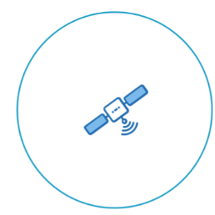
\includegraphics[width=.3\textwidth]{imgs/sat1}
             \caption{Un premier satellite}
             \label{fig:1sat}
         \end{figure}

         En se munissant d'un second satellite, de distance connue, on peut de la même manière tracer autour de sa position une boule de rayon égal à cette distance.

         \begin{figure}[h]
             \centering
             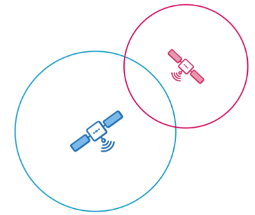
\includegraphics[width=.3\textwidth]{imgs/sat2}
             \caption{Deux satellites}
             \label{fig:2sat}
         \end{figure}

         Et finalement, la même opération sur un troisième satellite permettra au récepteur d'identifier l'unique point d'intersection entre les boules, correspondant à sa position.

         \begin{figure}[h]
             \centering
             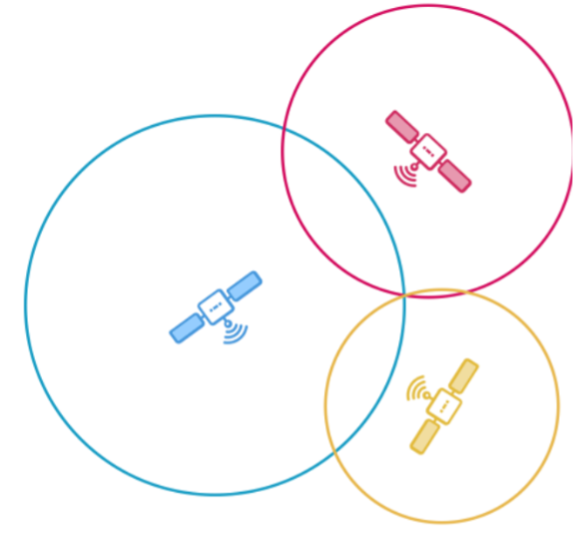
\includegraphics[width=.3\textwidth]{imgs/sat3}
             \caption{3 satellites, détermination de position}
             \label{fig:3sat}
         \end{figure}

         Il est alors très logiquement possible d'affiner ce résultat en augmentant le nombre de satellites, ou encore la précision de la mesure du temps du récepteur par exemple.

         \begin{figure}[h]
             \centering
             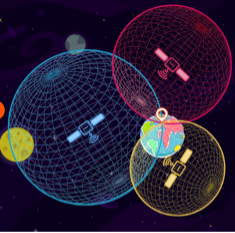
\includegraphics[width=.5\textwidth]{imgs/sat-3D}
             \caption{Représentation en 3D}
             \label{fig:repr3d}
         \end{figure}

      \subsubsection{Synchronicité des horloges}
         La détermination de la distance entre le récepteur et les satellites étant intrinsèquement liée à un repère d'horloge, une synchronisation temporelle entre les satellites et le récepteur est nécessaire (une erreur de l'ordre du millionième de seconde entraîne une erreur de positionnement de l'ordre de la centaine de mètres !).

         Pour résoudre ce problème, un quatrième satellite est nécessaire, permettant de se munir d'une donnée temporelle précise (grâce à son horloge atomique embarquée), permettant alors au récepteur de compenser les différences d'horloge afin d'affiner son positionnement jusqu'à en obtenir une valeur précise et juste~\cite{gebre-egziabherGNSSApplicationsMethods2009}.

      \subsubsection{Facteurs influençant le positionnement par satellite}
         Il est cependant à noter que divers facteurs tels que le niveau d'humidité, les variations de pression ou encore le rayonnement solaire peuvent modifier la vitesse ou la direction des signaux émis par les satellites, introduisant des erreurs dans les mesures.

         On comprend donc l'utilité de se munir d'un grand nombre de satellites afin de s'assurer d'une bonne précision.

   \subsection{Lecture de données GNSS}\label{subsec:lecture-de-donnees-gnss-format-nmea}
      \subsubsection{Format NMEA}
         Le format NMEA (\textit{National Marine Electronics Association}) a été proposé en 1983 par la marine nationale américaine afin de permettre la standardisation des communications entre les équipements marins, dont les émetteurs / récepteurs GPS\@.
         Ce format permet d'échanger facilement diverses informations de positionnement et de calibrage entre plusieurs appareils, faisant \textit{de facto} du format NMEA une norme pour les différents GNSS~\cite{hofmann-wellenhofGNSSGlobalNavigation2007}.

      \subsubsection{Lecture d'une trame NMEA}
         Une trame NMEA débute nécessairement par un symbole \texttt{\$} directement suivi du système GNSS reçu (GP pour le GPS, GL pour le GLONASS\dots) et l'intitulé de la donnée (code de 5 lettres).
         Suivent alors, séparées par des virgules, les données reçues.

         On donne l'exemple d'une trame GGA reçue par le système GPS, et on remarquera en particulier le \textit{checksum}, clé de contrôle permettant de vérifier la validité des données :

         \begin{figure}[h]
             \centering
             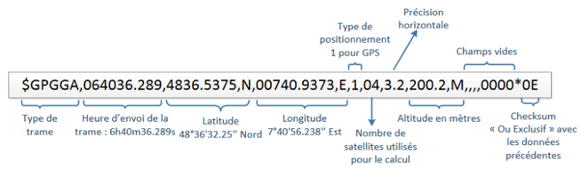
\includegraphics[width=.95\textwidth]{imgs/trame-gga}
             \caption{Exemple de trame GGA}
             \label{fig:trame-gga}
         \end{figure}
